\chapter{\label{sec:easyspinsim}EasySpin simulations}

\begin{figure}[H]
    \centering
    \begin{subfigure}[b]{0.3\textwidth}
        \centering
        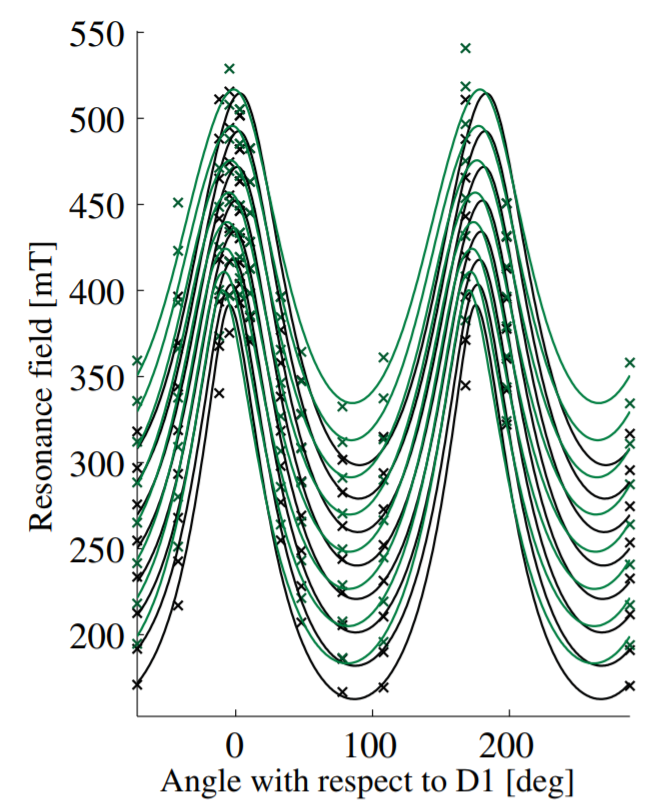
\includegraphics[width=\textwidth]{NdflaigrespectD1}
        \caption{Rotation (360 $^{\circ}$)
around crystal b axis ($\phi$ = 69.83 $^{\circ}$, $\theta$
= 3.75 $^{\circ}$)}
    \end{subfigure}
%     \hfill
    \begin{subfigure}[b]{0.3\textwidth}
        \centering
        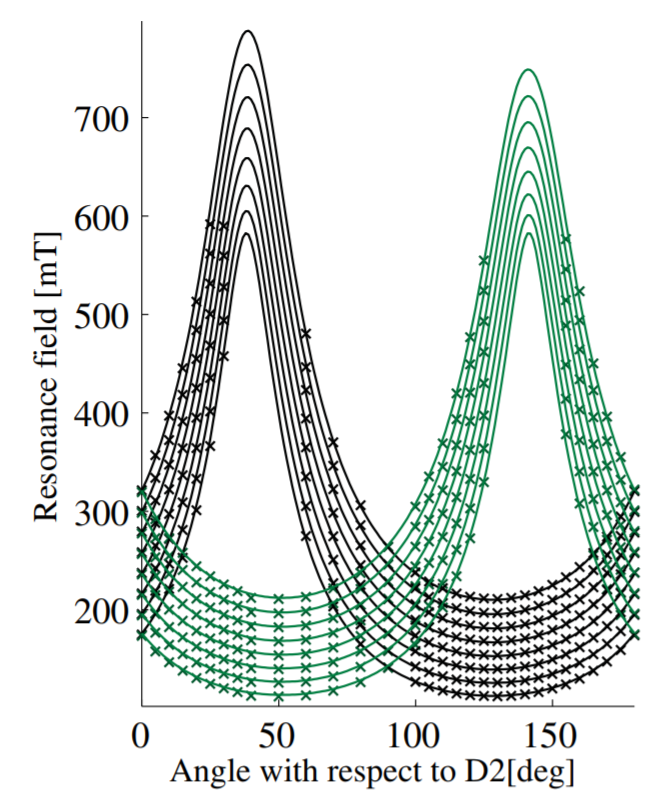
\includegraphics[width=\textwidth]{NdflaigrespectD2}
   \caption{Rotation (180 $^{\circ}$)
around crystal D1 axis
($\phi$ = 189.13 $^{\circ}$, $\theta$= 96.21 $^{\circ}$)}
   \end{subfigure}
      \begin{subfigure}[b]{0.3\textwidth}
        \centering
        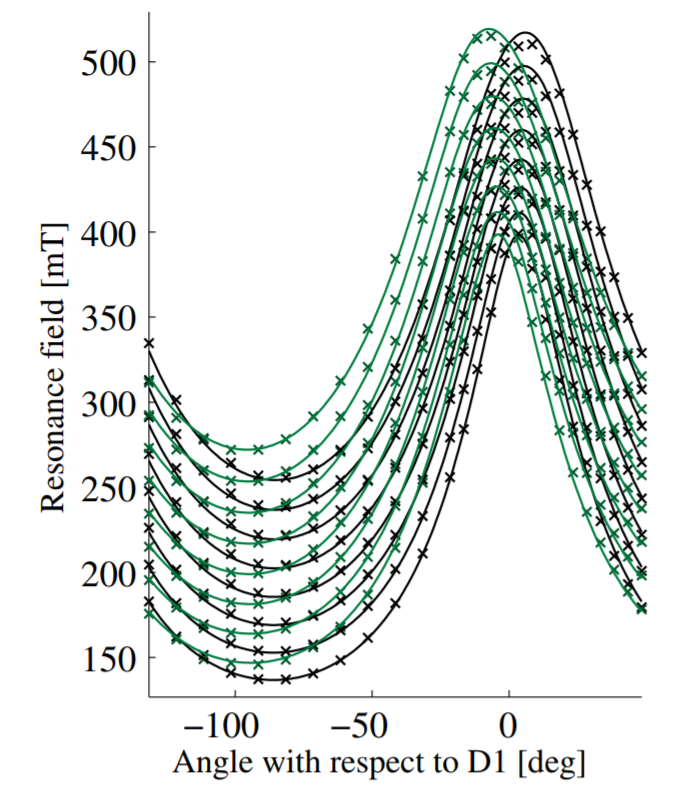
\includegraphics[width=\textwidth]{NdflaigrespectD12}
   \caption{Rotation (180 $^{\circ}$)
around crystal D2 axis
($\phi$ = 89.72 $^{\circ}$, $\theta$
= 92.77 $^{\circ}$)}
   \end{subfigure}
   \caption{Angular variation of the hyperfine resonance fields of both sub sites (green and
black) for $145$Nd$^{3+}$ doped YSO. Experimental values (cross) and fit (line). Copy from Ref.\citep{mairflaig}.}
   \label{fig:mairflaigthesis}
    \end{figure}
    
    \begin{figure}[H]
    \centering
    \begin{subfigure}[b]{0.45\textwidth}
        \centering
        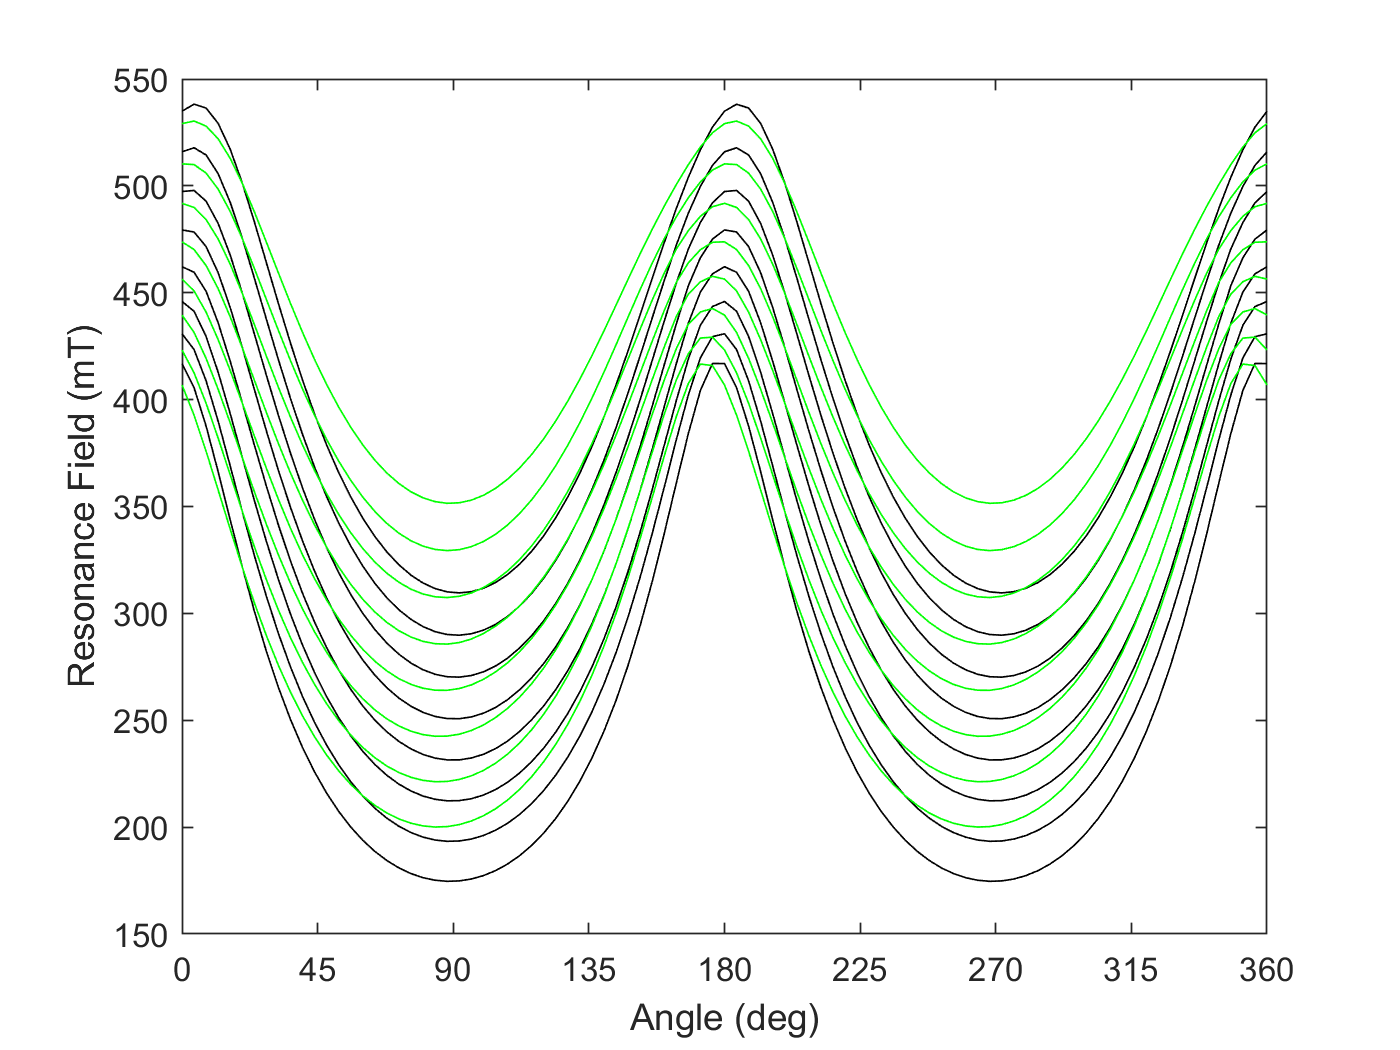
\includegraphics[width=\textwidth]{crystalbaxis}
        \caption{Rotation (360 $^{\circ}$)
around crystal b axis ($\phi$ = 69.83 $^{\circ}$, $\theta$
= 3.75 $^{\circ}$)}
    \end{subfigure}
%     \hfill
    \begin{subfigure}[b]{0.45\textwidth}
        \centering
        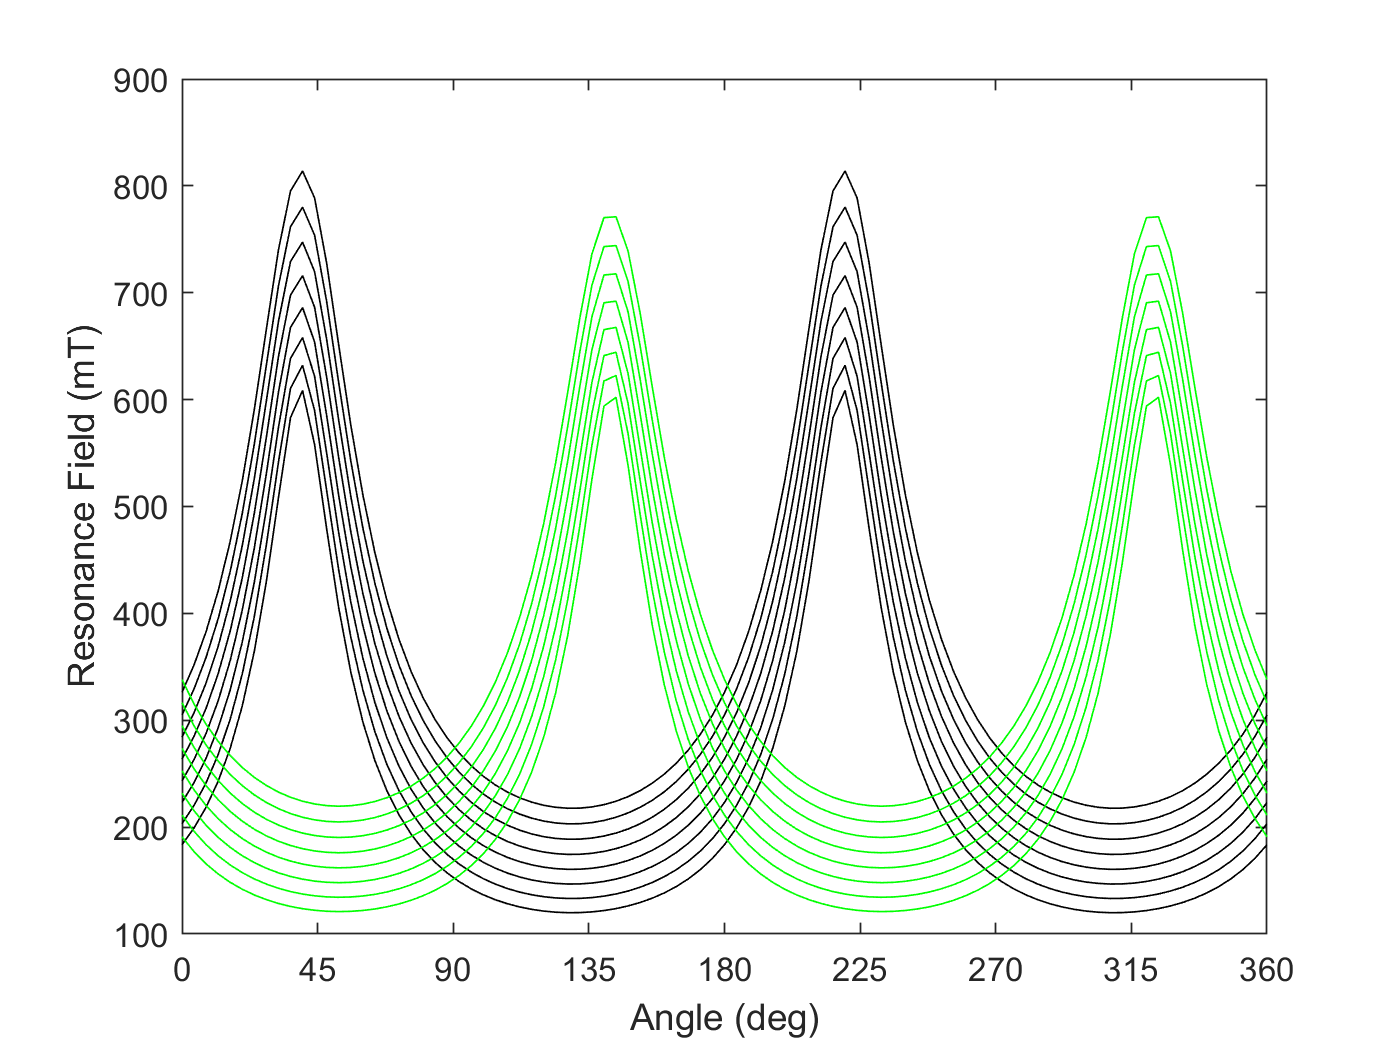
\includegraphics[width=\textwidth]{crystalD1axis1}
   \caption{Rotation (360 $^{\circ}$)
around crystal D2 axis
($\phi$ = 89.72 $^{\circ}$, $\theta$
= 92.77 $^{\circ}$)}
   \end{subfigure}
      \begin{subfigure}[b]{0.45\textwidth}
        \centering
        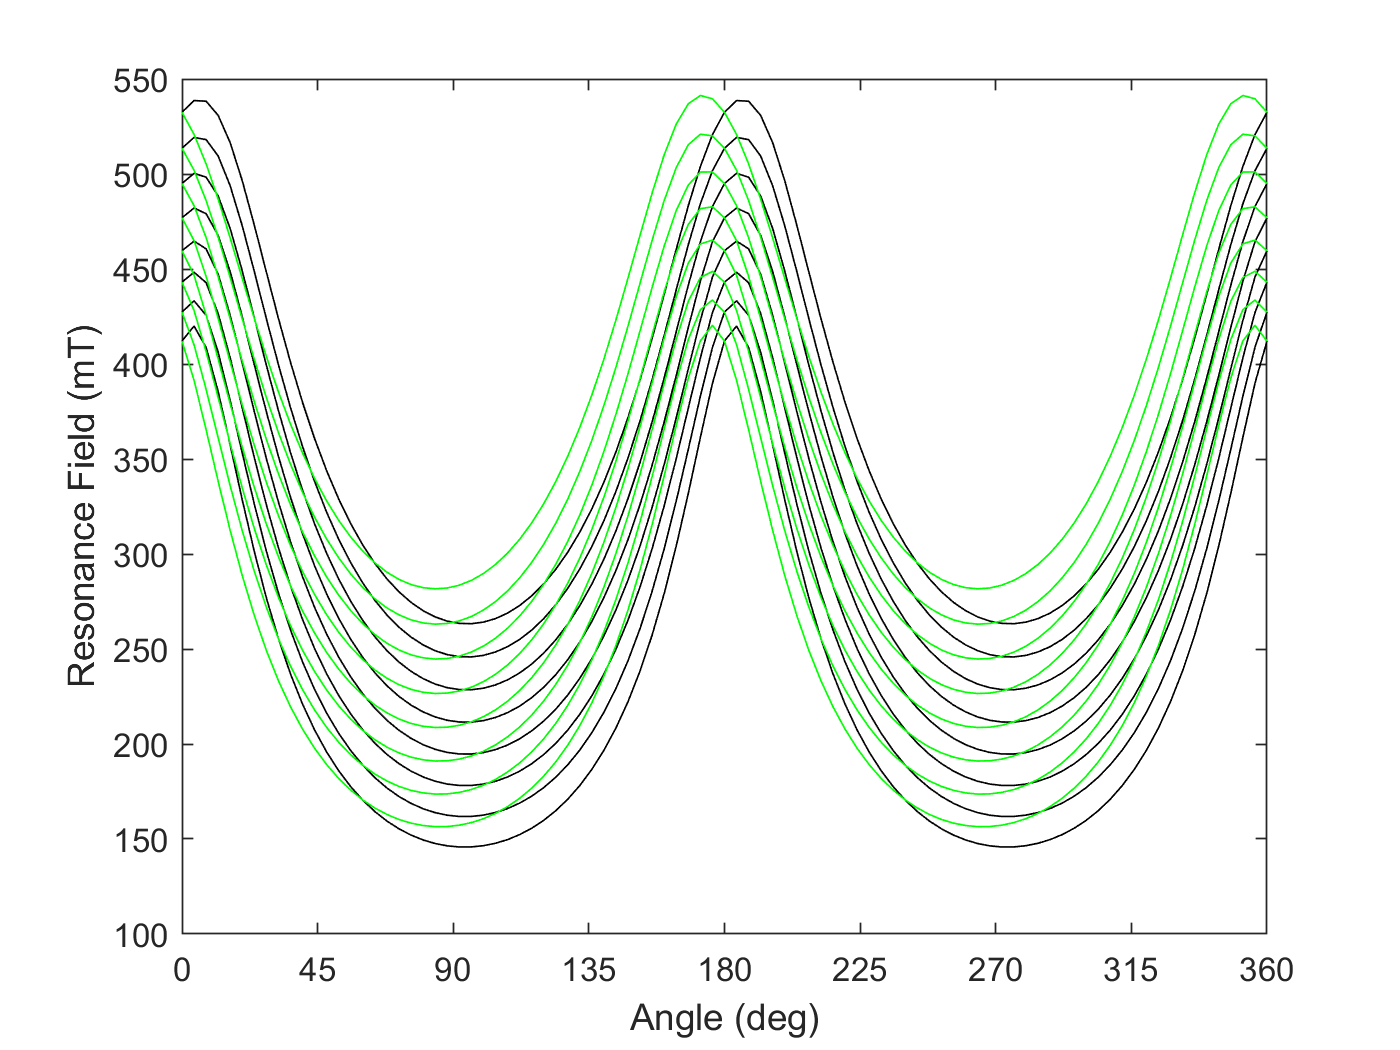
\includegraphics[width=\textwidth]{crystalD2axis}
   \caption{Rotation (360 $^{\circ}$)
around crystal D2 axis
($\phi$ = 89.72 $^{\circ}$, $\theta$
= 92.77 $^{\circ}$)}
   \end{subfigure}
   \caption{Simulation of the angular variation of the hyperfine resonance fields of both sub sites (green and
black) for $145$Nd$^{3+}$ doped YSO.}
   \label{fig:mairflaigthesisreplicate}
    \end{figure}


